% !TEX root = ../../thesis.tex

\section{Head aesthetic design} % (fold)
\label{sec:head-design}
Lot of effort have been put in the design and aesthetic of Poppy's head (see \figurename~\ref{fig:poppy_beta_head}) because it is  both its identity and main communication apparatus.
On an aesthetic point of view, its design was inspired of course by existant robots, but also by animals, objects and arts. The main inspiration insight are displayed as a board on the \figurename~\ref{fig:head_inspiration}. We tried to achieve a design cute, expressive and among all simple.

\begin{figure}[p]
    \begin{center}
        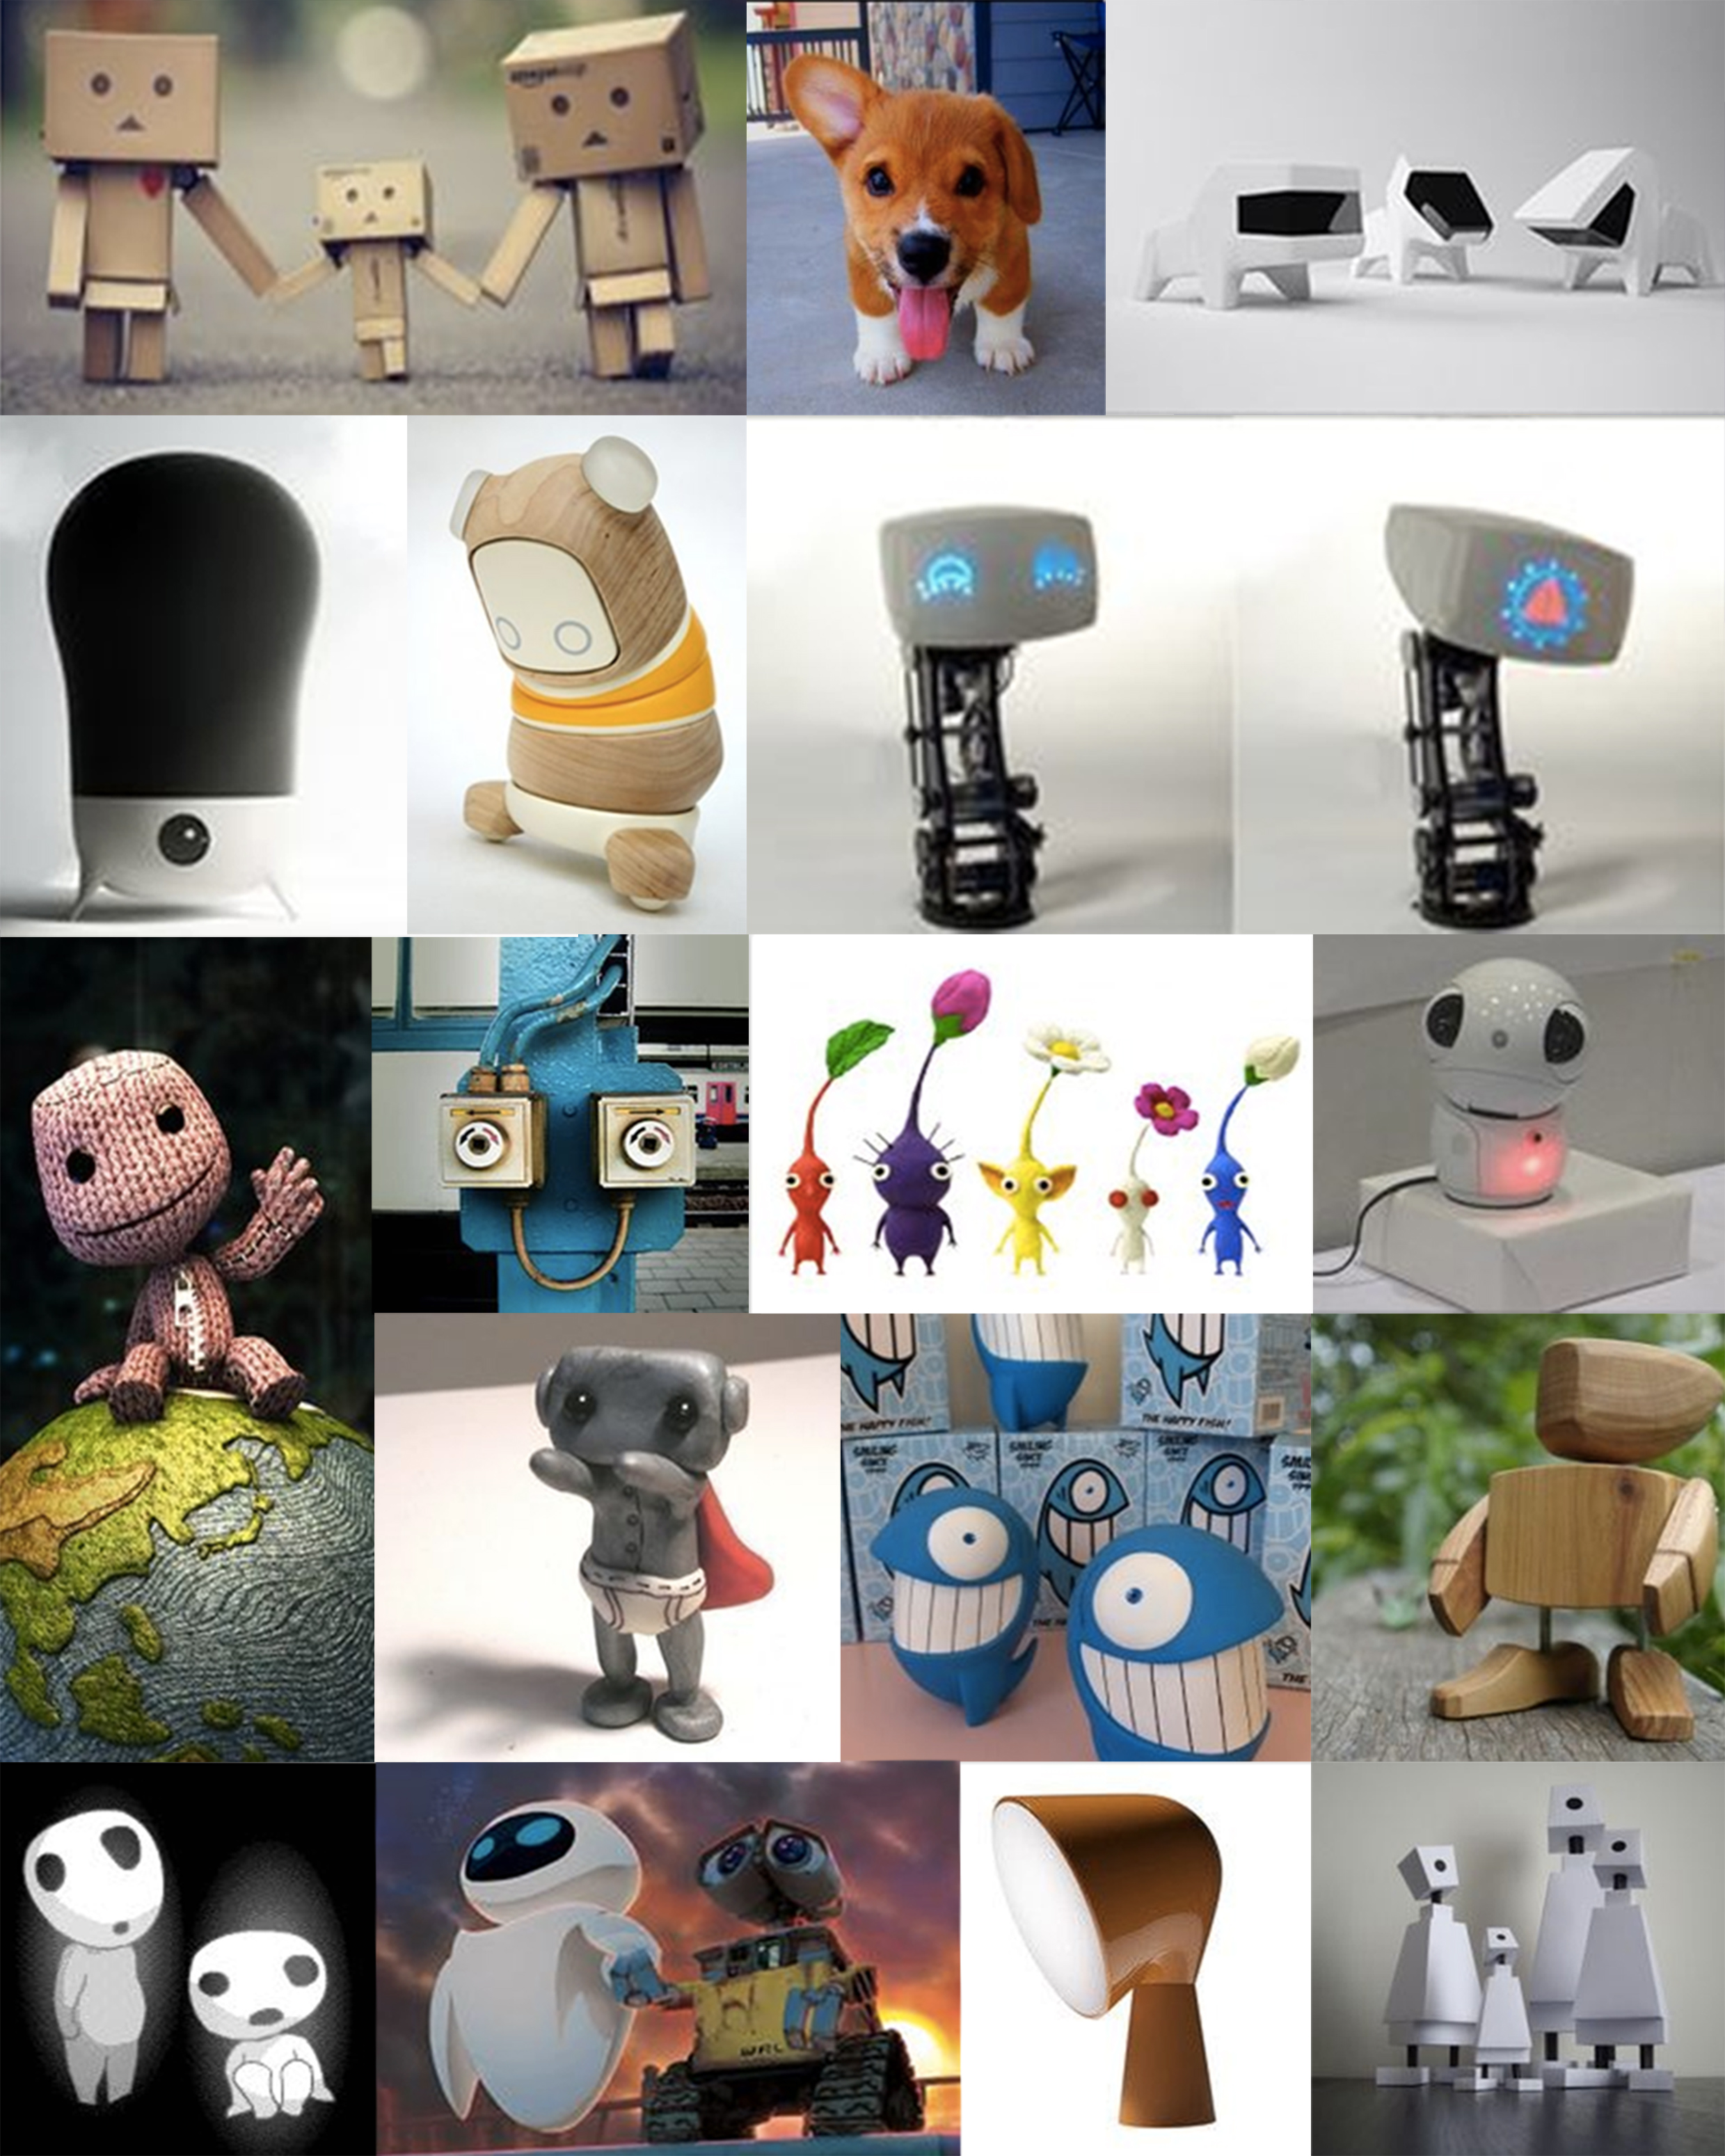
\includegraphics[width=\linewidth]{head_inspiration.jpg}
    \end{center}
    \caption{Complete board available on pinterest \url{http://www.pinterest.com/matthieulapeyre/robot/}}
    \label{fig:head_inspiration}
\end{figure}

Yet because of the multi-articulated vertebral column, Poppy has only free room in the head to embed all electronics components needed. Therefore strong technical constraints were imposed because the head has to embed all electronic architecture plus the communication sensorimotor apparatus composed by a wide 4.3" screen, cameras, and audio devices.
This components strongly constraints the design of the robot. Especially the screen, which requires a large flat part on the face. Obtaining a nice and rounded head shape with such constraints were rather difficult and require several iterations before obtaining a first correct finish (see \figurename~\ref{fig:poppy_beta_head}).

This process involved first few sketches that gave the main idea of the desired design. But the transfer to CAD modeling was quite complex, this kind of shape are rather difficult to design using parametric tools. The use of clay sculpting has been very helpful to go from the 2D drawing to the 3D shape.

\begin{figure}[p]
\centering
    \subfloat[][]{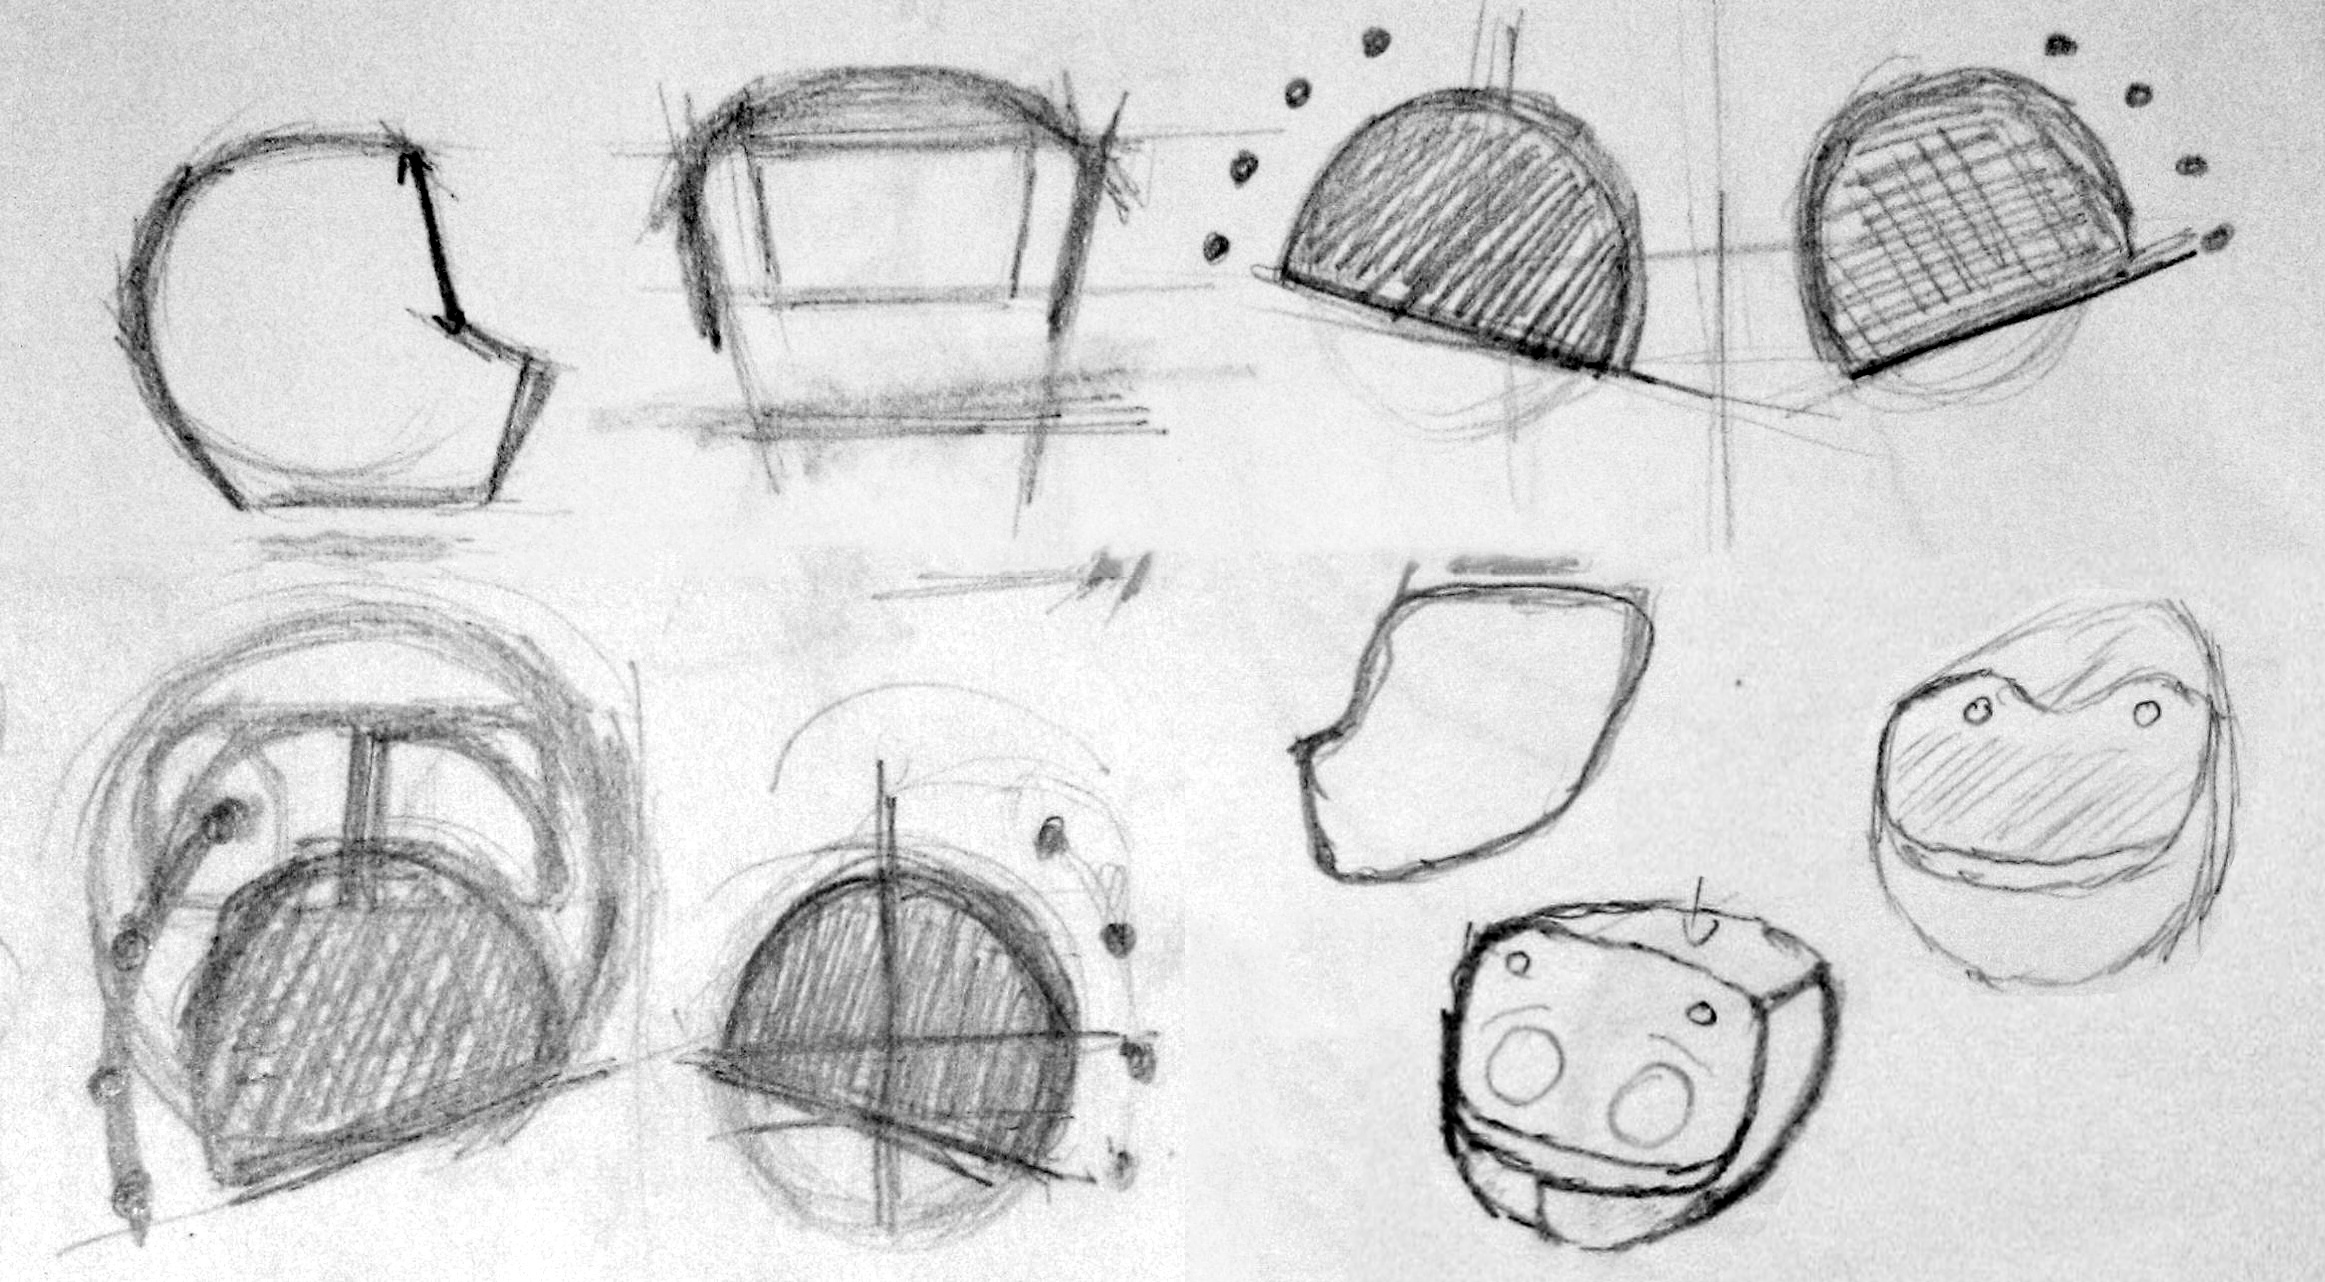
\includegraphics[height=4.5cm]{first_sketch.jpg}}
    \hfil
    \subfloat[][]{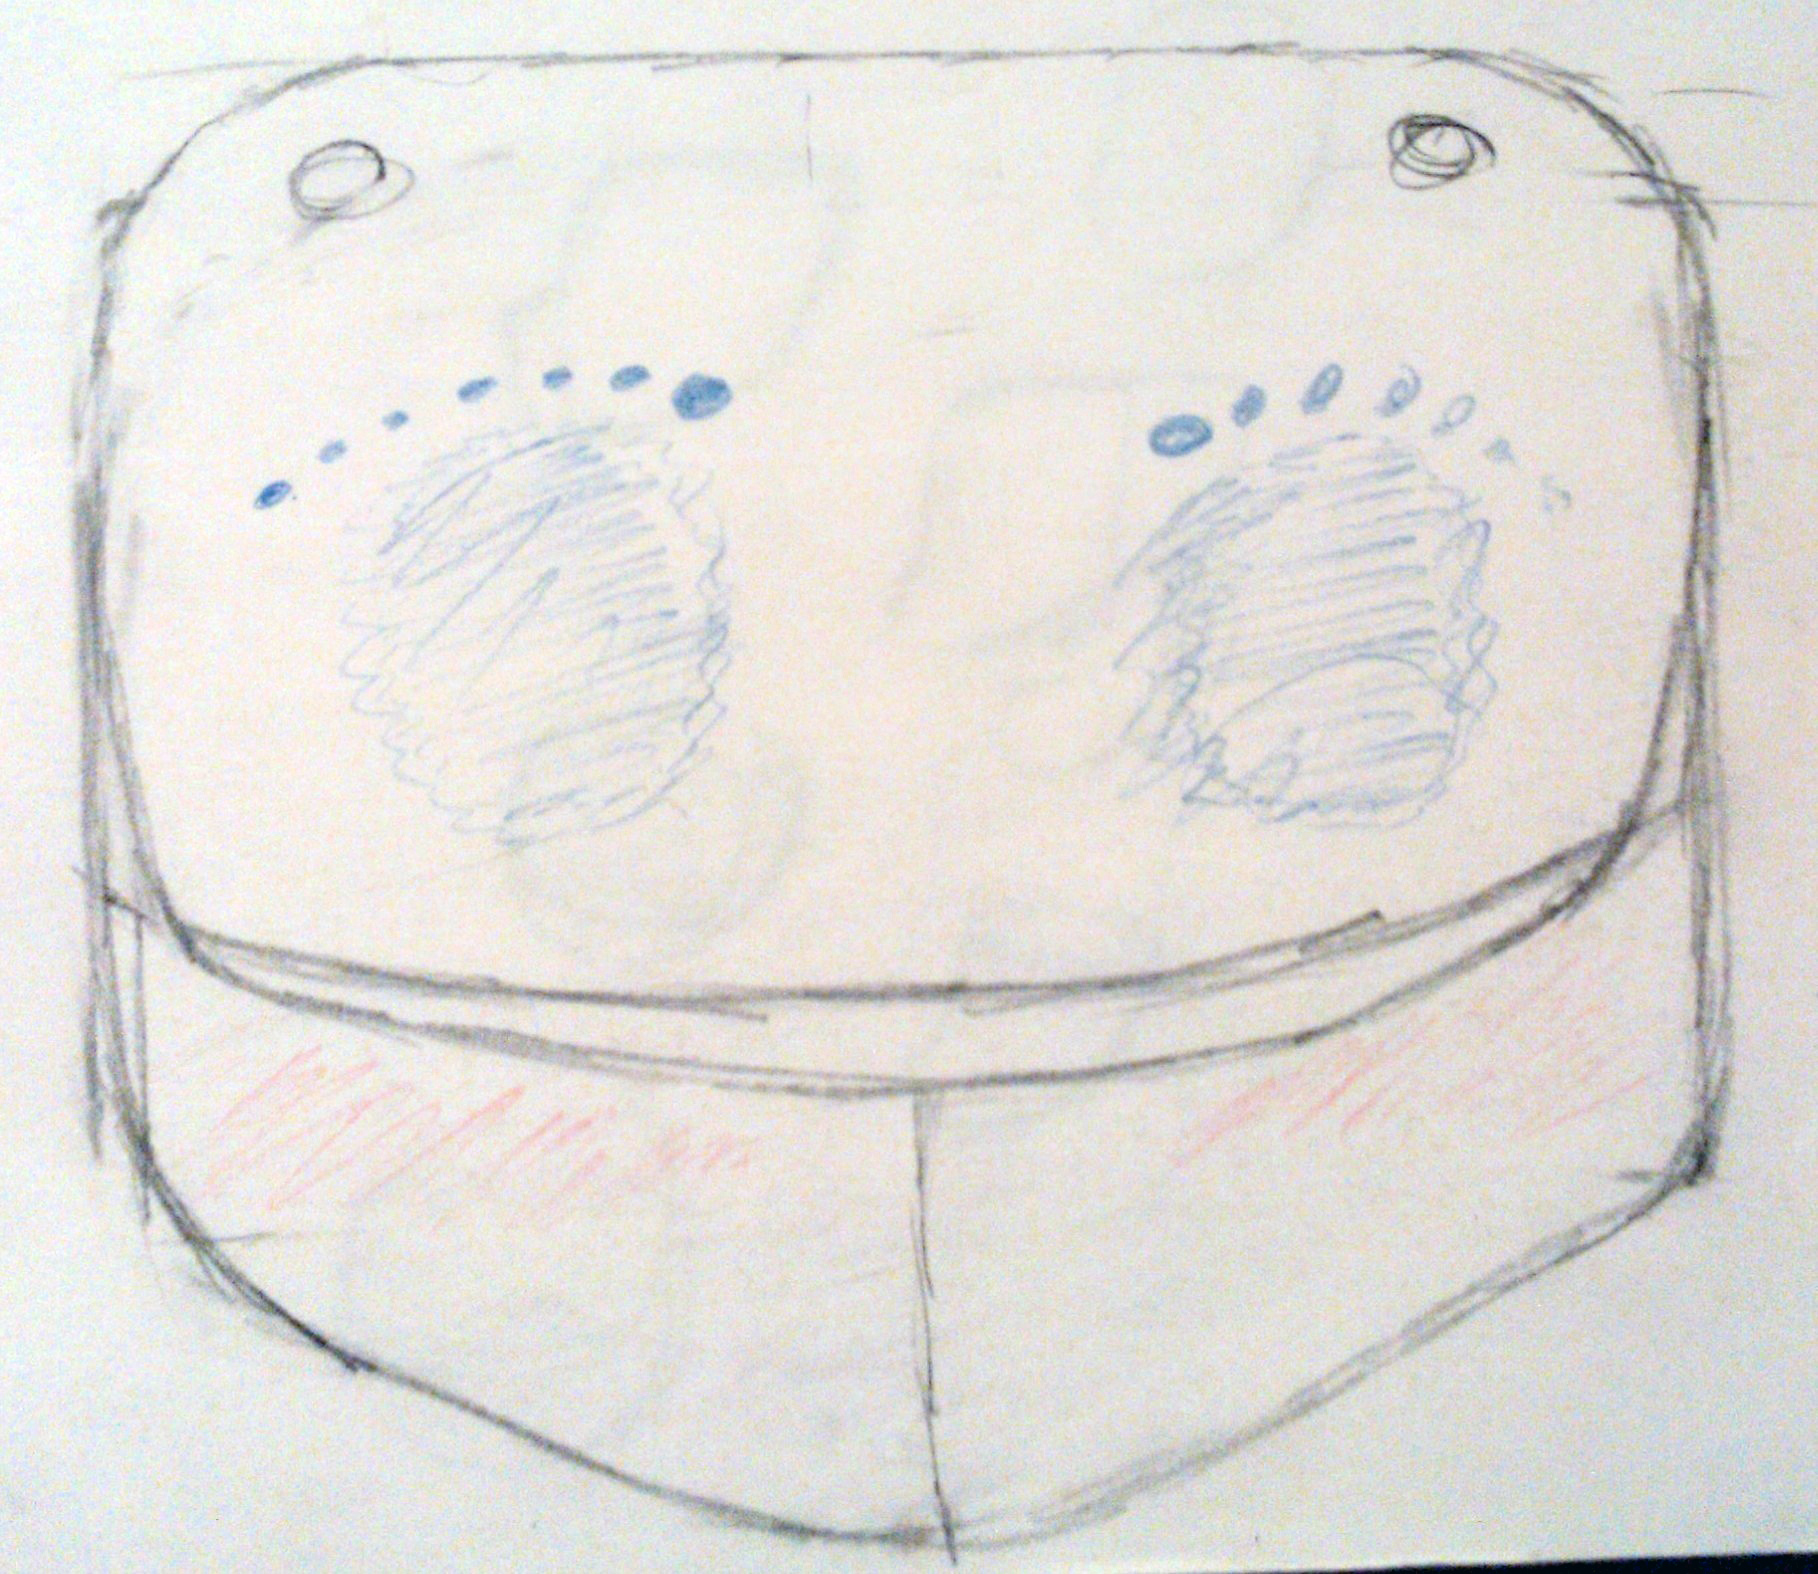
\includegraphics[height=4.5cm]{poppy_head_sketch.jpg}}
    \newline
    \subfloat[][First clay sculpture]{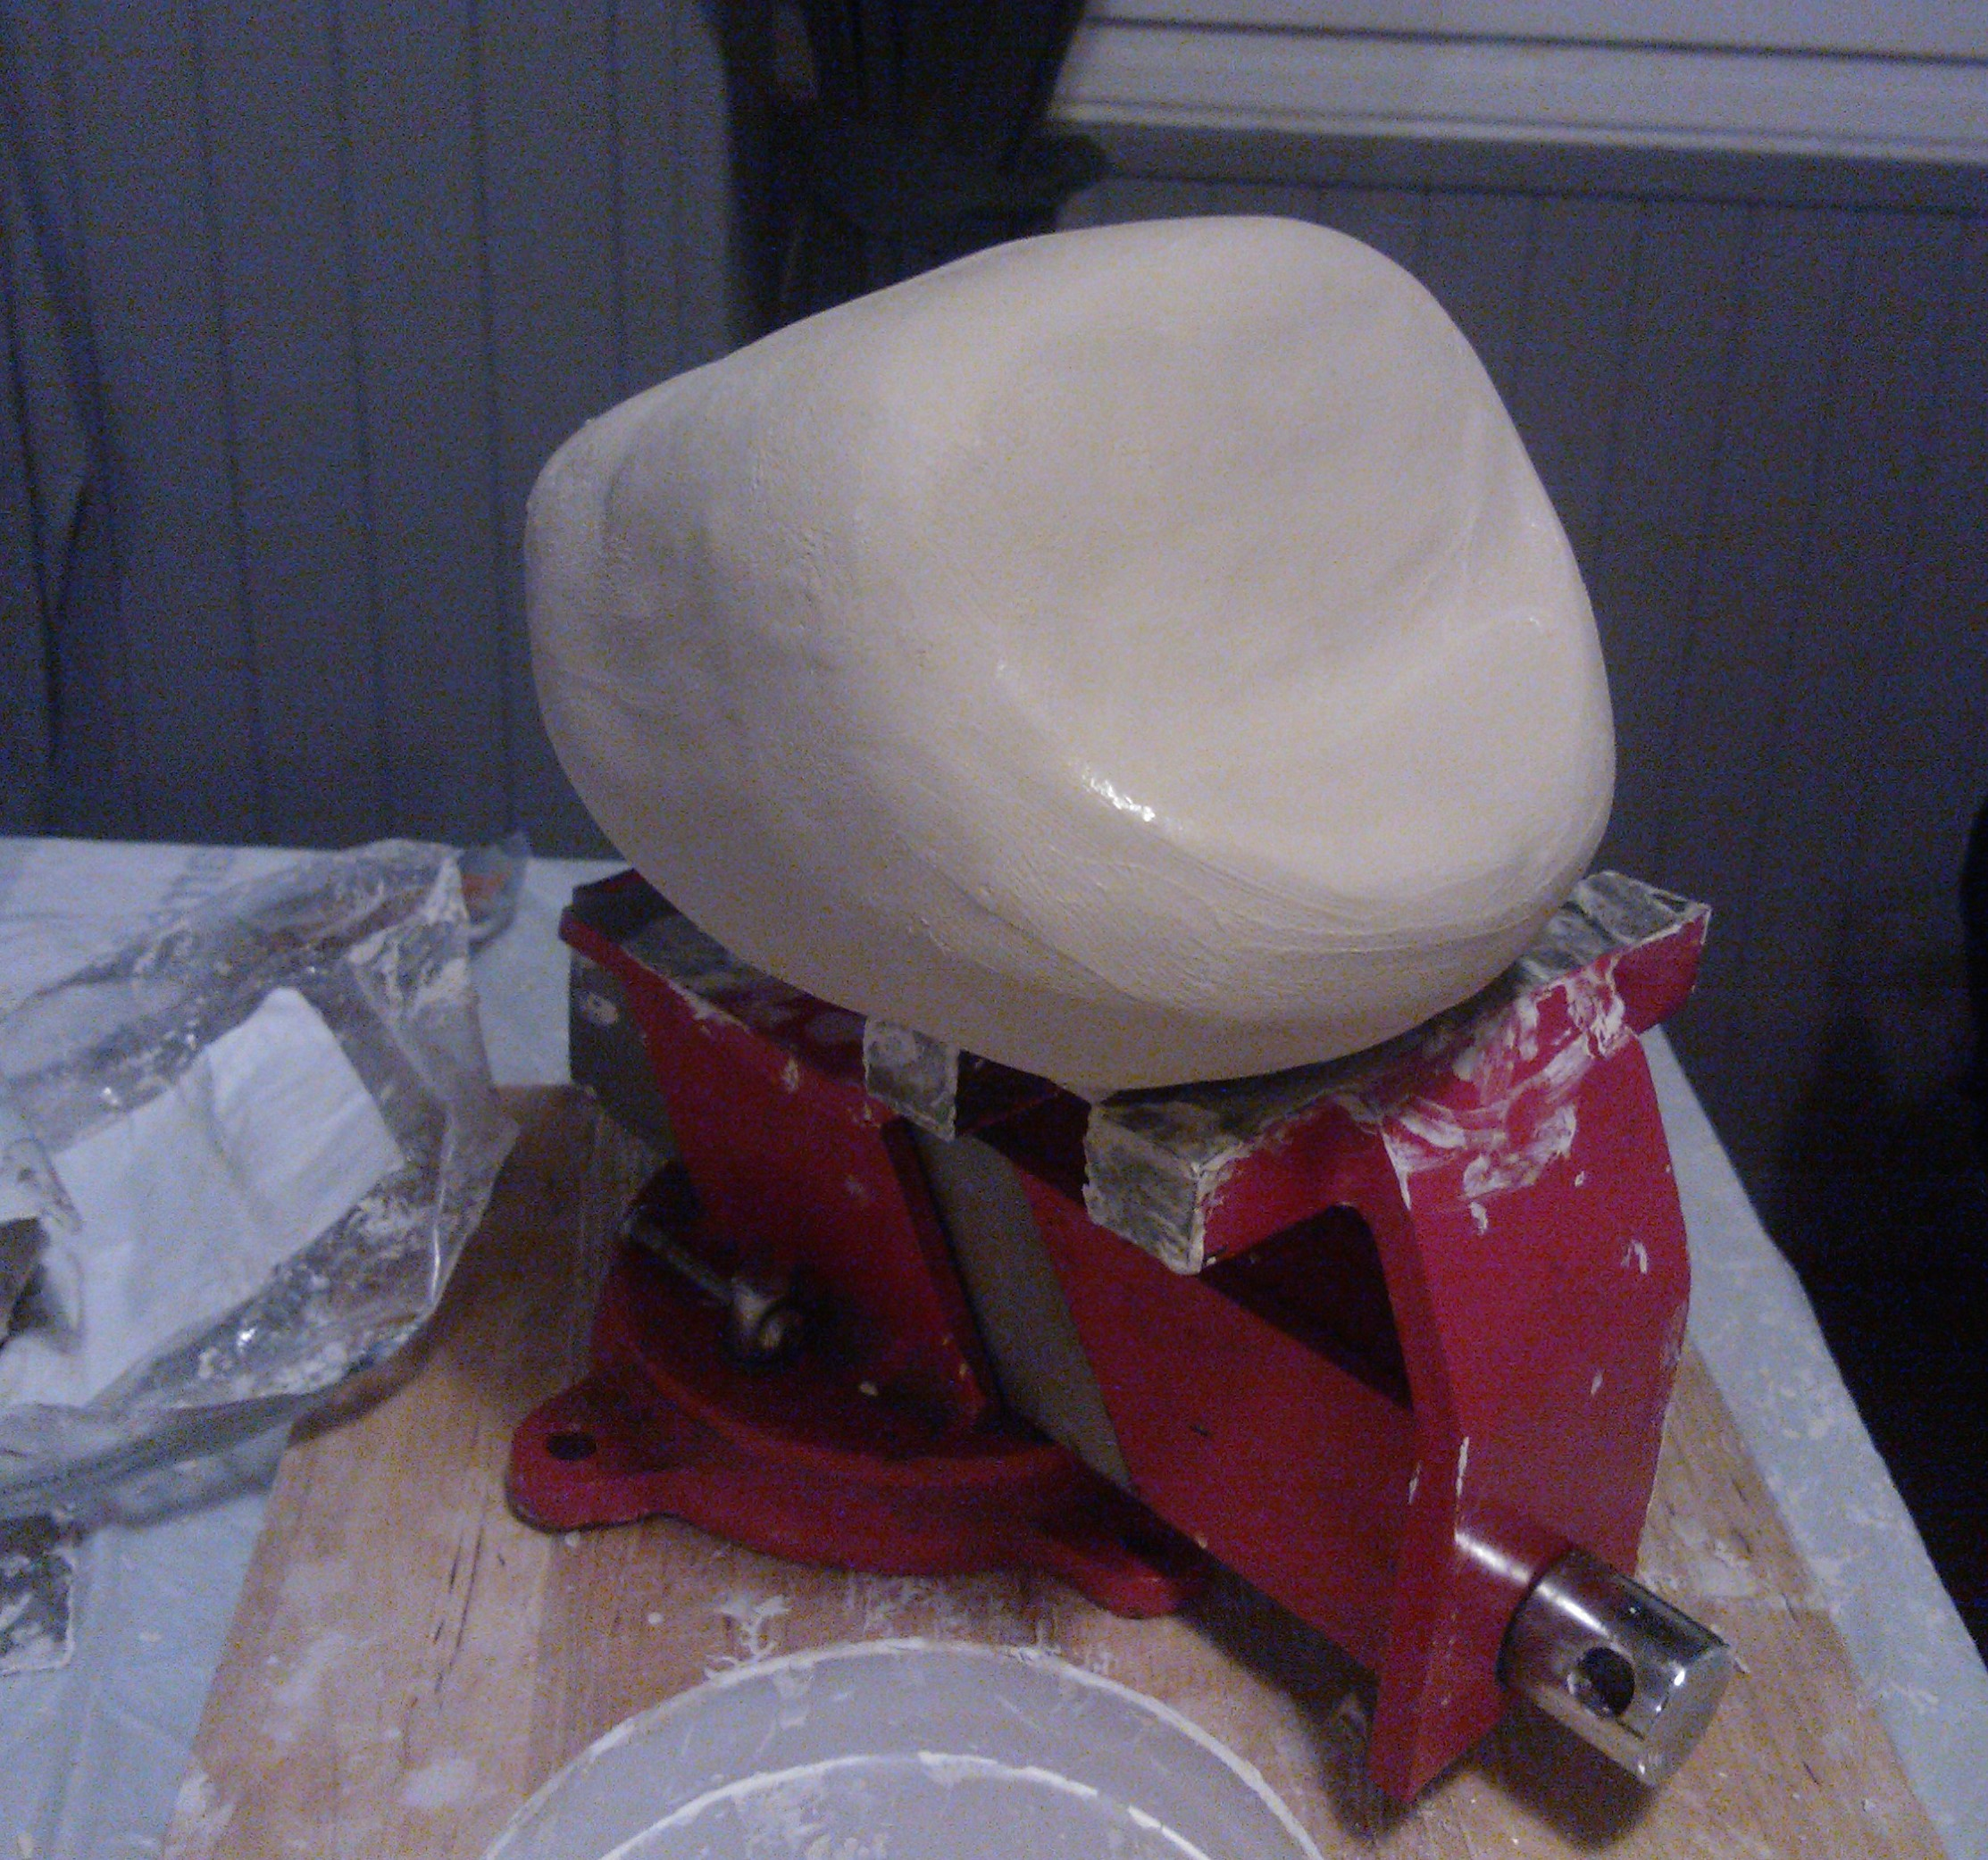
\includegraphics[height=5.5cm]{first_poppy_clay.jpg}}
    \hfil
    \subfloat[][First CAO model]{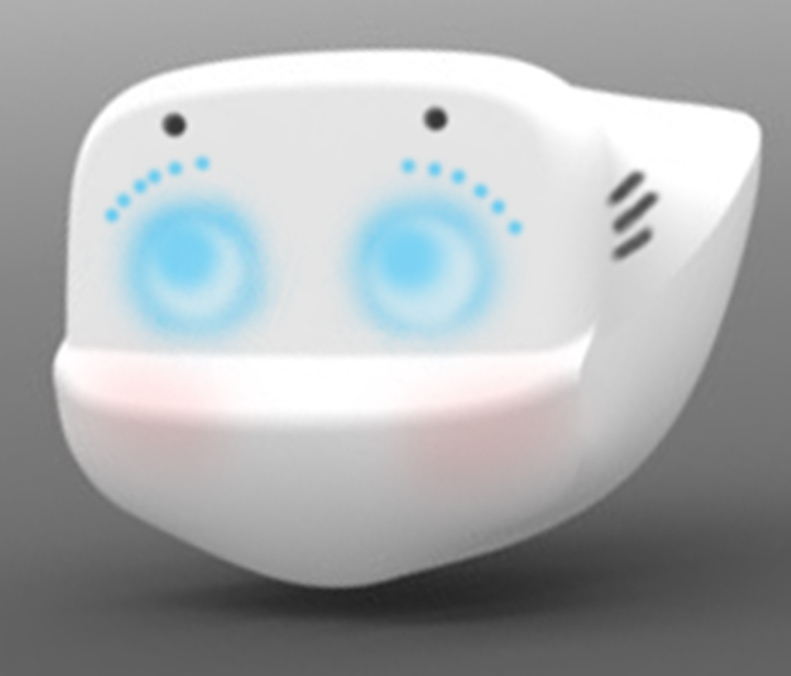
\includegraphics[height=5.5cm]{head_first_trial.jpg}}
    \newline
    \subfloat[][Poppy beta]{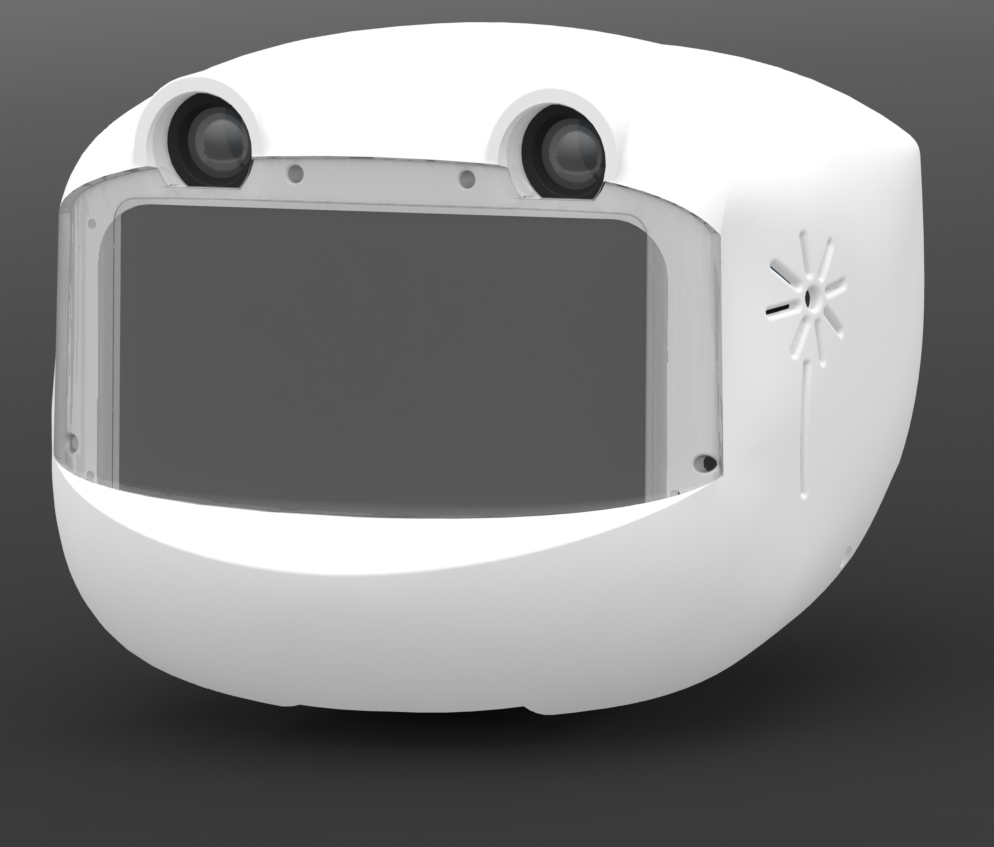
\includegraphics[height=5.5cm]{head_beta.jpg}}
    \hfil
    % \subfloat[][The first assembly]{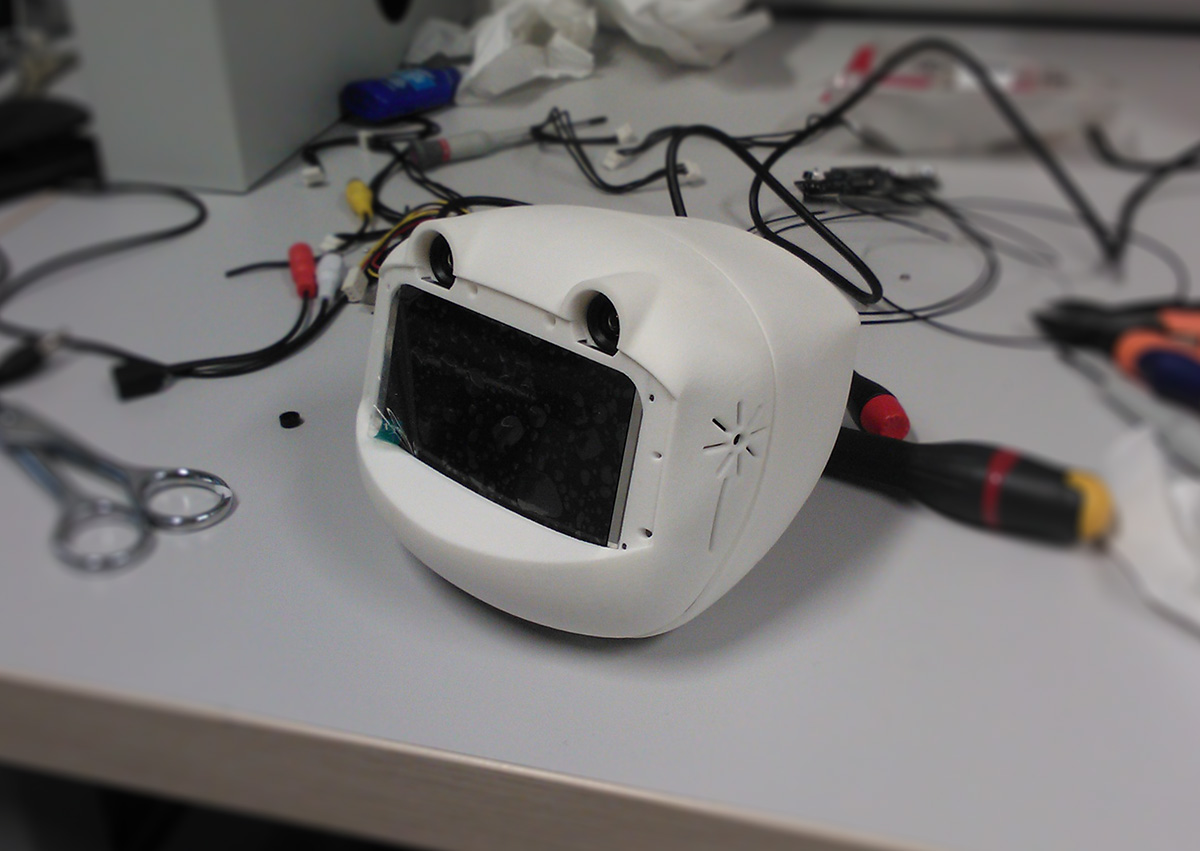
\includegraphics[height=5.5cm]{head_beta_assembled.jpg}}
    % \hfil
    \subfloat[][Screen powered on with basic eyes display]{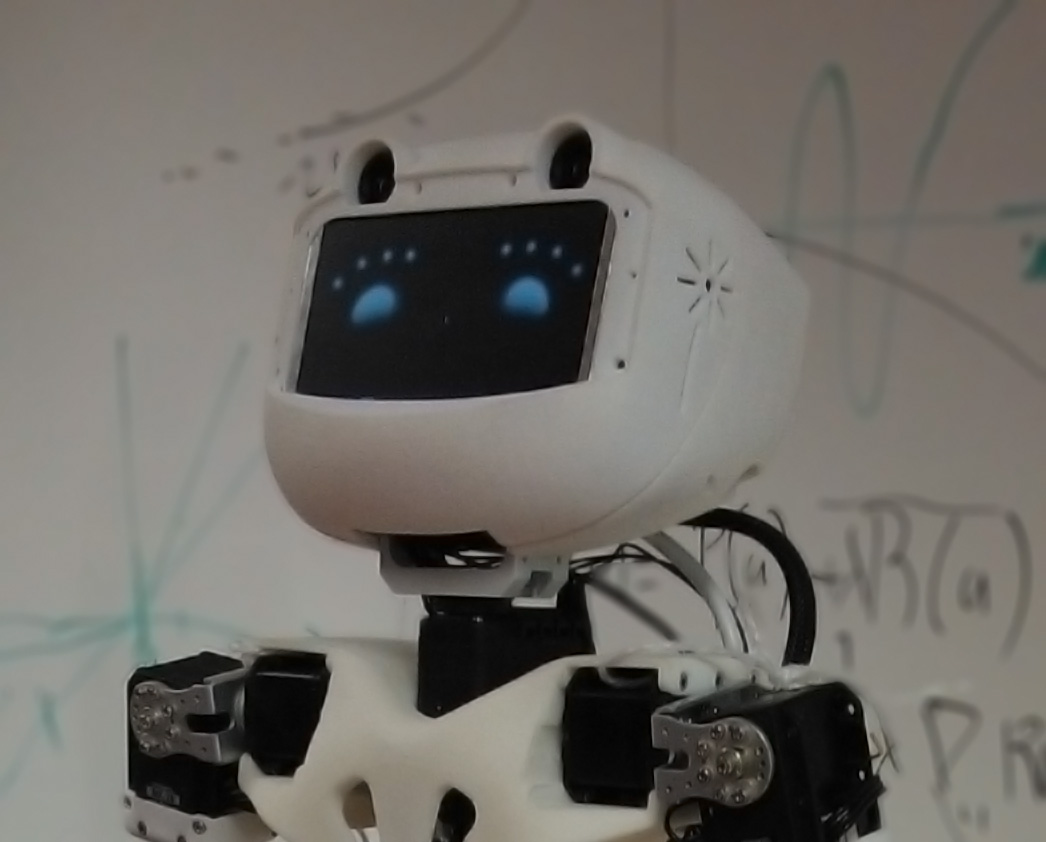
\includegraphics[height=5.5cm]{poppy_beta_eyes.jpg}}
    \caption{Evolution of Poppy head from the first sketches to the Poppy beta version.}
    \label{fig:head_sketch}
\end{figure}


However, in the first beta version showed in \figurename~\ref{fig:head_sketch}, there is a major design error. Indeed our desire was to have a screen to create and explore freely expressive eyes but the use of two visible cameras changed the way people saw Poppy's head. Of course, people seeing 2 cameras considers they are the eyes of the robot and therefore extrapolate that the screen may be the mouth or another face part.

We are currently working on the new design of Poppy's head and we simply addressed this issue by replacing the two big camera by a small one with a pinhole lens, which can be hidden on the Poppy face see \figurename~\ref{fig:poppy_head_v1}.

\begin{figure}[tb]
\centering
    % \subfloat[][Mix between Poppy beta 3D printed head and clay sculpture]{\includegraphics[height=5cm]{second_poppy_clay.jpg}}
    % \newline
    \subfloat[][Poppy 1.0]{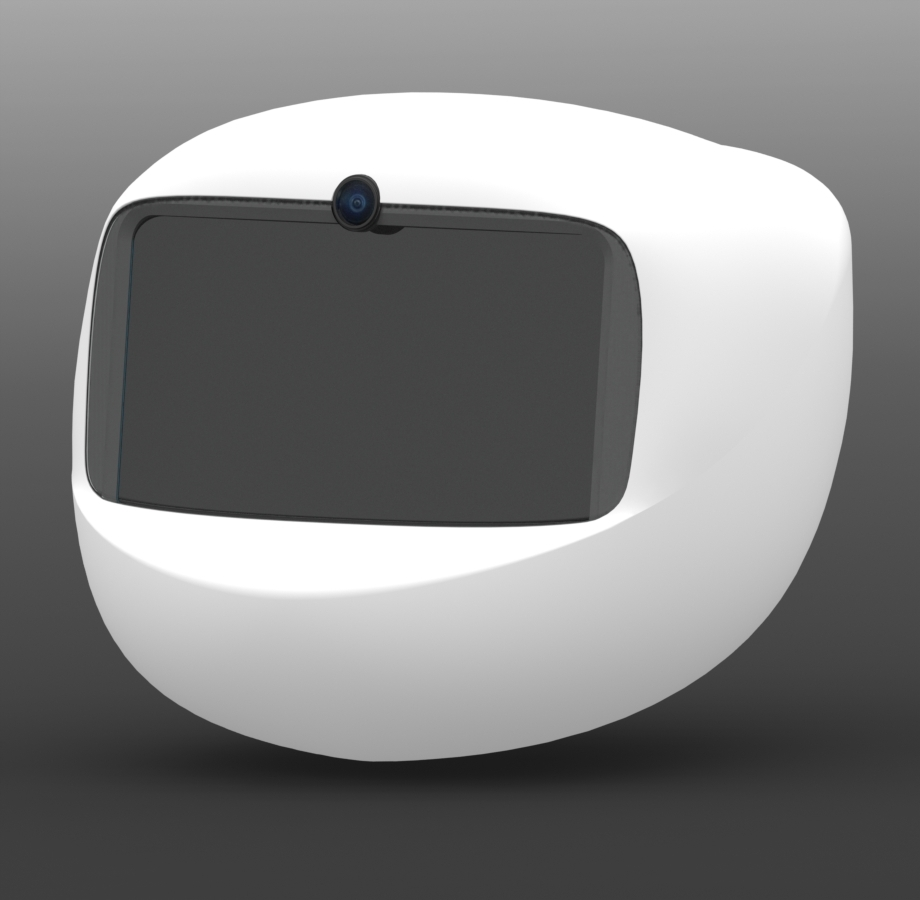
\includegraphics[width=0.5\linewidth]{poppy_v1_head.jpg}}
    \caption{}
    \label{fig:poppy_head_v1}
\end{figure}


While this work it is still in progress, we will update this section afterward with blueprint of the electronic integration and final design explanation.
